% !TeX spellcheck = de_DE
\documentclass[]{article}

\usepackage[utf8]{inputenc}
\usepackage[T1]{fontenc}
\usepackage[scaled]{beramono}
\usepackage{amssymb}
\usepackage{amsmath}
\usepackage{graphicx}
\usepackage[top=2cm, bottom=2cm, left=2cm, right=4cm]{geometry}
\usepackage{csquotes}
\usepackage{listings}
\usepackage{hyperref}
\usepackage{booktabs}

\lstset{
	tabsize=2,
	language=Java,
	showstringspaces=false,
	basicstyle=\footnotesize\ttfamily,
}

%no indentation
\setlength\parindent{0pt}

\pagestyle{empty}
\usepackage{wasysym}
\usepackage{multicol}

\begin{document}
	
	\section{Grammatiken}
	
	\begin{enumerate}
	\item Welche der Zeichenketten sind gültig bezüglich des abgebildeten Syntaxdiagramms?
	
	\begin{minipage}{0.4\linewidth}
	\begin{itemize}
		\item[$\square$] X
		\item[$\checked$] XX
		\item[$\checked$] XXXX
		\item[$\checked$] XXXXX
		\item[$\checked$] XXXXXXX
	\end{itemize}
	\end{minipage}
	\begin{minipage}{0.5\linewidth}
		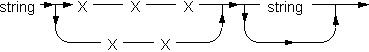
\includegraphics[width=\linewidth]{figures/syntax-string.png}
	\end{minipage}
	\vspace{2ex}
	
	\item Welche der Zeichenketten sind gültig bezüglich des abgebildeten Syntaxdiagramms?
	
	\begin{minipage}{0.4\linewidth}
		\begin{itemize}
			\item[$\checked$] 212
			\item[$\square$] 333
			\item[$\square$] 22394
			\item[$\square$] 0330
			\item[$\checked$] 6135798
		\end{itemize}
	\end{minipage}
	\begin{minipage}{0.5\linewidth}
		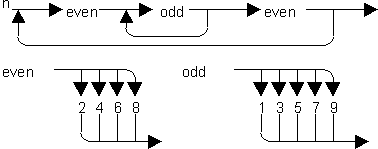
\includegraphics[width=\linewidth]{figures/syntax-evenodd.png}
	\end{minipage}
	\vspace{2ex}

	\item Überführen Sie die folgende Grammatik in EBNF in ein äquivalentes Syntaxdiagramm:
	
	\texttt{digitWithoutZero ::= '1' | '2' | '3' | '4' | '5' | '6' | '7' | '8' | '9'\\[1ex]
	digit ::= '0' | digitWithoutZero	\\[1ex]
	nat ::= digitWithoutZero \{digit\}\\[1ex]
	integer ::= ['-'] nat}
	
	\vspace{3ex}
	
	\begin{minipage}[t]{0.2\textwidth}
		\texttt{digitWithoutZero:}
		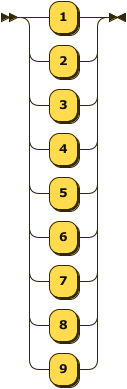
\includegraphics[scale=0.8]{figures/syntax-digitWithoutZero.png}
	\end{minipage}\hspace{1cm}
	\begin{minipage}[t]{0.3\textwidth}
		\texttt{digit:}\\
		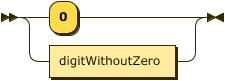
\includegraphics[scale=0.8]{figures/syntax-digit.png}
		
		\vspace{1cm}
		
		\texttt{nat:}\\
		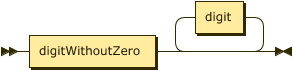
\includegraphics[scale=0.8]{figures/syntax-nat.png}
		
		\vspace{1cm}
		
		\texttt{integer:}\\
		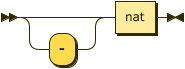
\includegraphics[scale=0.8]{figures/syntax-integer.png}
	\end{minipage}
		
		\vspace{30ex}
	
		\item Beschreiben Sie die Bildung von deutschen Zahlwörtern bis 9999 als EBNF.\\ Beispiel: Fünftausendsiebenhundertsechsunddreißig.
		
		\begin{lstlisting}[gobble=4]
		ZAHLEN_BIS_20 	::==	"EINS"|"ZWEI"|"DREI"|"VIER"|"FUENF"|"SECHS"|
													"SIEBEN"|"ACHT"|"NEUN"|"ZEHN"|"ELF"|"ZWOELF"|
													"DREIZEHN"|"VIERZEHN"|"FUENFZEHN"|
													"SECHSZEHN"|"SIEBZEHN"|"ACHTZEHN"|"NEUNZEHN"
		
		EINER						::== 	"EIN"|"ZWEI"|"DREI"|"VIER"|"FUENF"|"SECHS"|
													"SIEBEN"|"ACHT"|"NEUN"
		
		ZEHNER 					::== 	"ZWANZIG"|"DREISSIG"|"VIERZIG"|"FUENFZIG"|
													"SECHZIG"|"SIEBZIG"|"ACHTZIG"|"NEUNZIG"
		
		ZAHL_BIS_100 		::==	ZAHL_BIS_20 | ( [EINER "UND"] ZEHNER)
		
		STELLE3				 	::==	EINER "HUNDERT"
		
		STELLE4					::==	EINER "TAUSEND"
		
		ZAHLWORT 				::==	[STELLE4] [STELLE3] [ZAHL_BIS_100]
		\end{lstlisting}
		
	\end{enumerate}
	
	\section{Struktogramme}

	Geben Sie zu dem folgenden C-Segment ein äquivalentes Struktogramm an.
	
	\begin{multicols}{2}
	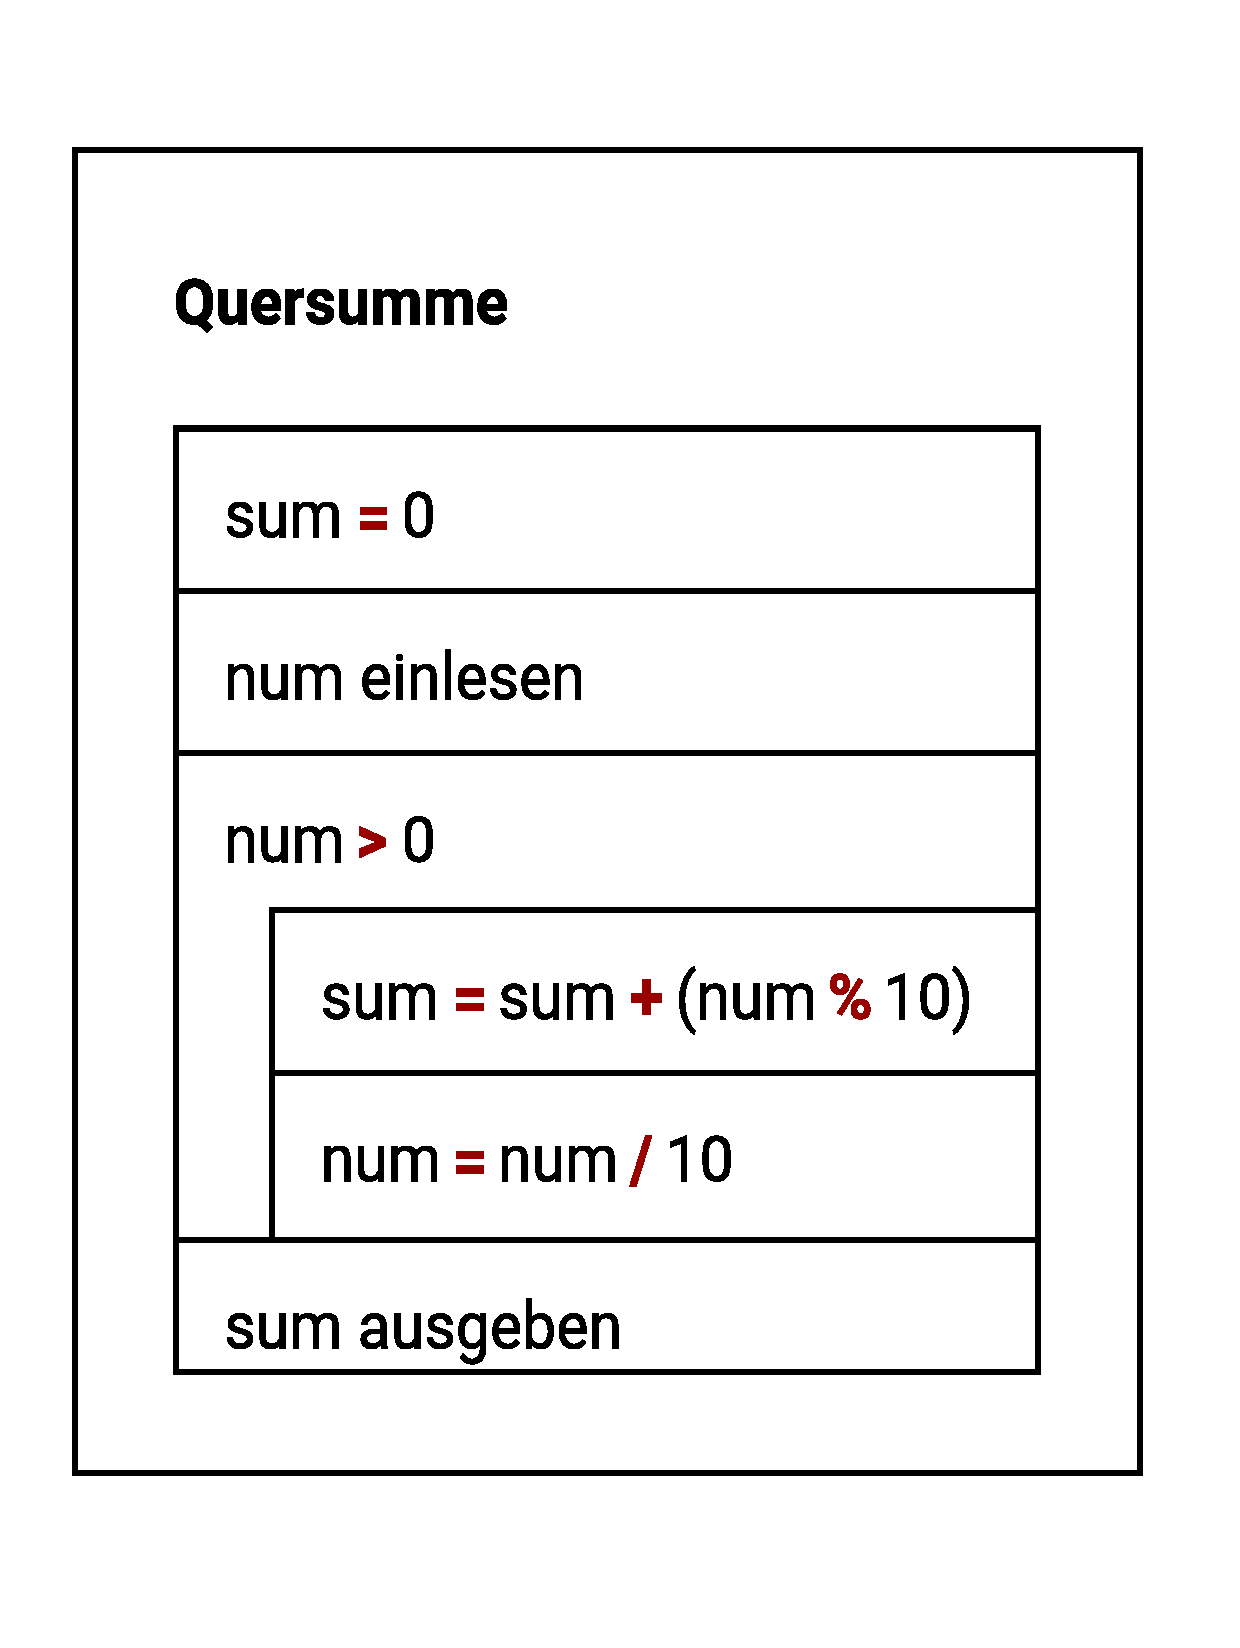
\includegraphics[scale=0.2]{figures/Quersumme}
	\columnbreak
	\begin{lstlisting}[gobble=4]
		int sum, num;
		sum = 0;
		scanf("%d", &num);
		while (num > 0) {
			sum = sum + (num % 10);
			num = num / 10;
		}
		printf("%d\n", sum);
	\end{lstlisting}
	\end{multicols}
	
	\section{Programmieren}
	
	Schreiben Sie ein Programm, das eine Temperatur in Grad Celsius einliest, dann in Fahrenheit umrechnet und beide Temperaturen ausgibt.
	Recherchieren Sie selbständig die Umrechnungsformel.\\
	\textit{Bonus: Das Ergebnis soll mit genau einer Nachkommastelle ausgegeben werden.}
	
	\begin{lstlisting}[gobble=4]
		#include <stdio.h>
		
		int main() {
		
			float c;
			
			printf("Bitte geben Sie eine Temperatur ein: ");
			scanf("%f", &c);
			
			float f = (c * (9.0/5.0)) + 32;
			
			printf("%.1f C sind %.1f F\n", c, f);
			
			return 0;
		}
	\end{lstlisting}
	
\end{document}